\chapter{Efficient solution of the linear systems}
\label{sec:solution-strategies}

When we combine implicit time integration schemes, a FEM spatial discretisation and the Newton-Raphson method for linearisation (as discussed in \cref{sec:time-discretisation,sec:galerk-meth-llg}) the result is a series of systems of linear equations which must be solved to obtain our approximate solution.
Additional or extended linear systems must be solved in the FEM/BEM for calculation of magnetostatic fields (as discussed in \cref{sec:hybr-finit-elem}).
In this \thisref{sec:solution-strategies} we discuss solution strategies for these systems.

In \cref{sec:llg-only-system} we first discuss the solution of the systems required in the calculation of the magnetostatic field assuming the magnetisation is known.
We then discuss methods of solving the linear system for the LLG equation assuming the magnetostatic field is known.

In \cref{sec:solut-coupl-syst} we introduce methods for the solution of the combined system: the LLG equation with magnetostatics, this is non-trivial because of the dense BEM matrix.
In particular: in \cref{sec:fully-implicit-bem} we introduce a novel approach which efficiently solves the coupled system while retaining all properties of the time integration scheme.

Finally in \cref{sec:numer-exper-fem-bem-systems} we present some numerical experiments comparing the approaches.


\section{Solution of decoupled systems}
\label{sec:llg-only-system}

In \thisref{sec:llg-only-system} we consider the separate solution of the magnetostatic and LLG problems.
Such methods are important building blocks for the solution of the coupled system.

First the linear system for the magnetostatic field calculations: the systems arising here are Poisson systems (\cref{sec:poisson-jacobian}) which are extremely well studied.
One efficent and robust method for solving Poisson systems on unstructured grids is to use the method of conjugate gradients (CG) with algebraic multigrid (AMG) as a preconditioner \cite[Chap. 2]{HowardElmanDavidSilvester2006}.
We implement such a solver using \oomph's implementation of CG with a relative convergence tolerance of $10^{-8}$.
As the preconditioner we use one V(1,1) cycle of \hypre's BoomerAMG preconditioner \cite{hypre} with Gauss-Seidel smoothing, CLJP coarsening and a connection strength threshold of $0.7$.

Note that the Poisson blocks $\Am$ are linear (the matrices do not depend on $\phim$, $\phione$ or $\mv$).
This means that when solving these matrices alone: 1) the Newton-Raphson iteration is not required (\ie the system will always be solved by a single iteration) and 2) the $\Am$ matrices can be computed once and stored for reuse throughout the duration of the simulation.


Now we focus on the linear systems resulting from the LLG equation.
There do not appear to be any efficient, robust and scalable solvers in the literature for this system with linearisation by the Newton-Raphson method.
% Typically a Krylov solve with an ILU preconditioner \cite{Suess2002} is used, ??ds: some people use direct multigrid, others use picard iteration ??ds this belongs in intro probably.
% This should work for sufficiently small time steps, \ie when the mass matrices of \cref{eq:llg-jacobian} are the dominant term, or when the number of nodes is sufficiently small.
% It would not be expected to work efficiently for larger time steps and large numbers of nodes.
Try two solvers in our model, unfortunately neither are expected to be scalable to large problem sizes with large time steps.

The first method used is a direct solve by LU decomposition (using the \superlu package \cite{superlu}).
As discussed in \cref{sec:direct-methods} this method is extremely robust but is very slow for large matrices, particularly for problems in three spatial dimensions.

The second method is to use GMRES preconditioned by an incomplete LU decomposition (ILU).
We \oomph's GMRES implementation with left preconditioning, no restarts and a relative convergence tolerance of $10^{-8}$.
For the ILU preconditioner we use \hypre's Euclid with one level of fill in and no drop tolerance.
Incomplete LU decomposition with no fill in was also tested but found to be ineffective, especially for larger time steps.
This method can be efficient for medium sized problems (up to around 100,000 nodes), but for larger problems the preconditioner is ineffective and slower to set up.
It is also not particularly robust: iteration counts can vary widely depending on problem parameters.

Unfortunately we have not had time to research more effective solvers for the LLG system.

\section{Solution of coupled LLG-magnetostatics systems}
\label{sec:solut-coupl-syst}
% ??ds rewrite

% I think most people use something like the second actually: use Krylov solve of sparse part as prec for dense part.\cite{Suess2002} \footnote{The paper is by the authors of \femme, Knittel2011 cites that paper for \nmag's approach, .. ??ds} d'Aquino uses quasi-Newton: drop dense part

% The first technique is to use an ad-hoc \emph{semi}-implicit time integration scheme in which the magnetostatic calculations are handled explicitly.

% The second technique is to use a preconditioned Krylov solver in combination with hierarchical matrix techniques in order to efficiently solve the monolithic, \ie fully-implicitly-coupled system.

We now need to consider the solution of the combined LLG and FEM/BEM magnetostatics systems.
However, unlike typical FEM computations, these linear systems are not entirely sparse.
The BEM matrix, $\bm$, (derived in \cref{sec:discretisation}) appears as a dense block in the Jacobian.
In this \thisref{sec:semi-implicit-bem} we describe two approaches to efficiently solve the linear system despite this dense block.

% There are numerous well understood linear solvers, such as those discussed in \cref{sec:solution-lin-sys}, which can be extremely efficient for large sparse systems.
% But, at least in their standard form, they are much less efficient for systems involving a dense block. ??ds what do I mean, LU decomposition: massive increase in nnz, multigrid inapplicable, Krylov solvers maybe...


The first approach is to replace our implicit time integration scheme with a somewhat ad-hoc semi-implicit version: we handle the magnetostatic calculation explicitly while the rest of the calculation is done implicitly.
This results in decoupled solves for $\phione$, $\phi$ and $\mv$ at each step, and the dense block only appears as a matrix-vector multiply.
However this means that we are no longer using the time integration methods discussed in \cref{sec:some-implicit-time-integrators}, instead we are using some new ad-hoc time integration scheme.
The stability, convergence and geometric integration properties of the original schemes do not necessarily carry over to the semi-implicit versions.

The second approach is to construct a linear solver which can efficiently handle the dense block.
We present a novel solver which consists of a Krylov solver combined with a block preconditioner, iterative subsidiary solves and a hierarchical representation of the BEM block.


??ds comment on what other people have done either here or in introduction


\subsection{Residuals and Jacobian for the coupled system}
\label{sec:bem-jacobian-structure}

As mentioned in \cref{sec:discretisation} the pair of Poisson equations for the FEM/BEM method are the same as those in \cref{sec:galerk-meth-llg} except for two differences.
The first difference is that there is no coupling from the auxilary potential $\phione$ to the LLG equations, and hence no corresponding $\Pm$ block.
The second difference is that there is an additional coupling, via the BEM matrix, between the boundary values of $\phione$ and the boundary values of $\phim$.

To enforce the Dirichlet boundary condition resulting from the collocation method BEM within the Newton solver we use the following simple residual
\newcommand{\rphimb}{\rphi_b}
\begin{equation}
  \rphimb(\phim_b, \phione_b) = \bm \phione_b - \phim_b,
\end{equation}
where $x_b$ denotes the vector of boundary values of $x$.
This simply enforces the condition $\phim_b = \bm \phione_b$ from \cref{eq:10}.

With the order of equations as: $\mv$, $\phim$, $\phione$ the Jacobian is then
\begin{equation}
  \Jm = 
  \begin{pmatrix}
    \Fm       & \Pm     &  \\
    \Qm'      & \Am' &  \bm'  \\
    \Qm       &         &   \Am
  \end{pmatrix},
  \label{eq:16}
\end{equation}
where the primed blocks are ones where the boundary and bulk values must be split up because of the BEM boundary condition:
\begin{equation}
  \Am' =
  \begin{pmatrix}
    \Am     & \pd{\phim}{\phim_b} \\
    0      & -\Idm  
  \end{pmatrix},
  \qquad
  \Qm' =
  \begin{pmatrix}
    \Qm \\
    0    
  \end{pmatrix}, 
  \qquad
  \bm' =
  \begin{pmatrix}
    0  & 0 \\
    0  & \bm 
  \end{pmatrix}.
\end{equation}


It is worth noting that a slightly different Jacobian struture could be obtained by modifying the derivation in \cref{sec:appl-magn-calc}.
Instead of using $\phim = \phione + \phitwo$ to eliminate $\phitwo$, we could use $\hms = - \grad ( \phione + \phitwo)$ and eliminate $\phim$.
This would result in both of the potentials having a $\Pm$ block, but only one of them having a $\Qm$ block.
It would also reduce the diagonal dominance of $\bm$.
We have not experimented with this alternative formulation.

The linear system to be solved at each Newton step is (see \cref{sec:newt-raph})
\begin{equation}
  \jac \corr = -\resi,
  \label{eq:87}
\end{equation}
where $\resi$ is the vector of the current discrete Newton residuals for $\mv$, $\phim$ and $\phione$ and we need to find the Newton update $\corr$.


\subsection{The semi-implicit approach}
\label{sec:semi-implicit-bem}

The first approach to the solution of the linear system \cref{eq:87} is to break it into multiple decoupled systems.
The idea is to use the fact that the magnetostatic fields are typically much weaker than the exchange field, so we hope that the stability of the problem will not be affected by switching to explicit magnetostatic calculations.


For the step from time $t_n$ to $t_{n+1}$ the basic algorithm is as follows 
\begin{enumerate}
\item Extrapolate $\phim_n$, $\phim_{n-1}$ to $t_{n+1}$ to get $\hat{\phim}_{n+1}$.
\item Use $\hat{\phim}_{n+1}$ to calculate $\mv_{n+1}$ (using an implicit time integration method, Newton-Raphson, LLG matrix solve).
\item Calculate $\phione_{n+1}$ using $\mv_{n+1}$ (Poisson solve).
\item Use boundary values of $\phione_{n+1}$ to get $\phim_{n+1}$ on the boundary (BEM matrix-vector multiply).
\item Calculate $\phim_{n+1}$ everywhere using the dirichlet boundary conditions given by 4. and $\mv_{n+1}$ (Poisson solve).
\end{enumerate}

For step 1 we must use a second order accurate extrapolation in order to ensure that the local truncation error of the overall time integration remains second order.
A simple second order extrapolation formula (based on Lagrange interpolation \cite[312]{Kincaid2002}) is 
\begin{equation}
  \label{eq:65}
  f(t_{n+1}) = \frac{t_{n+1} - t_n}{t_{n-1} - t_n}f(t_{n-1}) + \frac{t_{n+1} - t_{n-1}}{t_n - t_{n-1}}f(t_n).
\end{equation}
After substituting in $t=t_{n+1}$, $t_1=t_n$ and $t_0=t_{n-1}$ this gives an expression for $\hat{\phim}_{n+1}$
\begin{equation}
  \label{eq:66}
  \hat{\phim}_{n+1} = \frac{-\dtx{n+1}}{\dtn} \phim_{n-1} + \frac{\dtx{n+1} + \dtn}{\dtn} \phim_n.
\end{equation}
Note that if we are using the implicit midpoint rule we need to extrapolate $\phim$ to the midpoint rather than $t_{n+1}$, hence we use $\dtx{n+1} = \dtx{n+1} /2$ in the above equation.

Also note that starting this method requires magnetostatic potential values at two initial times. 
These values can be generated by directly calculating the potentials if the magnetisation values at two initial times are known.
Otherwise the first can be calculated from the initial condition and the potential at a second time can be calculated by taking a small time step and using a first order extrapolation formula.


The linear systems resulting from step 2. are for the LLG equation alone, and similarly the linear systems in step 3 and 4 are for the decoupled Poisson equations.
The solution of these systems proceeds exactly as discussed in \cref{sec:llg-only-system}.




\subsection{The fully implicit approach}
\label{sec:fully-implicit-bem}

??ds mention semi-implicit + iteration approach?

The alternative to the semi-implicit approach is to find an efficient way to solve the full system \cref{eq:16}, this is known as a ``monolithic'' method.
The difficulty is that the system contains a dense block, meaning firstly that the LU decomposition of J is ``very dense'' and secondly that any operations (\eg multiplication) on J will be significantly slower than for a sparse matrix ($\order{N + N_b^2}$ rather than $\order{N}$).
We use a combination of techniques to try to make this solve efficient.

The first and most important technique is the use of a Krylov solver, this has two benefits
Firstly the inverse (or LU decomposition, or ...) of the matrix is never computed, meaning that the denseness of the inverse has no effect.
Secondly, using a Krylov solver rather than a direct solve or a multigrid-based solver means that all that is required of $\jac$ is the computation of matrix-vector products.
This allows us to split $\jac$ into separate matrices as
\begin{equation}
  \jac = \jac_{\textrm{sparse}} + \Gm'',
\end{equation}
where $\Gm''$ contains only the dense block $\Gm$ and $\jac_{\textrm{sparse}}$ is sparse.
The matrix-vector product can be computed as
\begin{equation}
  \jac \xv = \jac_{\textrm{sparse}}\xv + \Gm''\xv,
\end{equation}
\ie the dense and sparse parts can be stored and used completely independently.

This leads us to the second component of our method: the use of a hierarchical matrix format for the dense BEM block $\Gm$ \cite{Borm2003,Forster2003,Knittel2011}.
This format reduces the computational cost for a matrix-vector product for the dense block to $\order{N_b \log N_b}$.
Since the number of boundary nodes $N_b$ is typically less than the total number of nodes in the problem this can allow the cost of matrix-vector products of $\jac$ to be optimal, \ie $\order{N}$ depending on the geometry.
It also reduces the memory requirements to $\order{N_b \log N_b}$.
The use of such formats is now fairly common in the application of the hybrid FEM/BEM method to micromagnetics problems.

The third and final component in our efficient solver is a cheap and effective preconditioner for the linear system.
Some approaches to such a preconditioner are discussed in the following section.


\subsubsection{Preconditioning strategies}
\label{sec:bem-solver-strategies}

\newcommand{\preca}{\mathcal{P}}
\newcommand{\precb}{\mathcal{Q}}
\newcommand{\precc}{\mathcal{R}}


\newcommand{\inexact}[1]{\widetilde{#1}}
\newcommand{\parinexact}[1]{\hat{#1}}
\newcommand{\pbin}{\inexact{\precb}}
\newcommand{\pcin}{\inexact{\precc}}




In this section we give a number preconditioning approaches for the monolithic system \cref{eq:16}.
The aim is to construct a preconditioner which give a (roughly) constant number of GMRES iterations independently of $N$, but which is also quick to set up and does not consume significant amounts of memory.

The first preconditioner is very simple: we do a direct solve (using LU decomposition) of the sparse part of $\Jm$, \ie
\begin{equation}
  \preca = 
  \begin{pmatrix}
    \Fm       & \Pm     &  \\
    \Qm'       & \Am'    &   \\
    \Qm       &         &   \Am
  \end{pmatrix}.
\end{equation}
This preconditioner, while more efficient than a direct solve including the dense block, still suffers from all the usual problems associated with a direct solver (\ie expensive in both memory and computation time when $N$ is large).
However, we are interested in its properties as a test of the effectiveness of dropping the $\Gm'$ block from the preconditioner.

Our second and third preconditioners are more ambitious: we drop additional blocks in order to make the preconditioner block triangular.
It can then be solved by inverting the diagonal blocks (exactly or approximately) and using back/forward substitution.
These preconditioners are
\begin{equation}
  \precb = 
  \begin{pmatrix}
    \Fm       &           &  \\
    \Qm'       & \Am'&   \\
    \Qm       &           &   \Am
  \end{pmatrix},
  \qquad
  \precc = 
  \begin{pmatrix}
    \Fm       & \Pm       &  \\
    & \Am' &   \\
    \Qm       &           &   \Am
  \end{pmatrix},
  \label{eq:ms-block-prec-drop-p}
\end{equation}
where $\precc$ can obviously be reordered to give a block triangular preconditioner.

However inverting $\precb$ or $\precc$ directly would still require an expensive direct solve of the three diagonal blocks $\Fm$, $\Am'$ and $\Am$.
Ideally we want to approximate these inverses by some cheap iterative process instead.

Based on the fact that CG preconditioned with AMG is known to be extremely effective for Poisson problems we test the use of an AMG preconditioner for the $\Am$ blocks (recall that CG and GMRES are both Krylov solvers, so the requirements for effective preconditioners are very similar).
Using this approximation we define two partially-inexact preconditioners, where we use $\inexact{x}$ to denote an iteratively solved approximate and $\parinexact{x}$ to denote a partially iterative (\ie with some direct solve still needed) preconditioner
\begin{equation}
  \parinexact{\precb} = 
  \begin{pmatrix}
    \Fm       &           &  \\
    \Qm'       & \inexact{\Am'} &   \\
    \Qm       &           &   \inexact{\Am}
  \end{pmatrix},
  \qquad
  \parinexact{\precc} = 
  \begin{pmatrix}
    \Fm       & \Pm       &  \\
    & \inexact{\Am'} &   \\
    \Qm       &           &  \inexact{\Am}
  \end{pmatrix}.
  \label{eq:ms-block-prec-drop-p}
\end{equation}

We also test the effect of approximating the $\Fm$ block using ILU-1, but we expect similar restrictions on the matrix size and time step size to those discussed in \cref{sec:llg-only-system}.
Using this approximation in addition to the AMG approximation to the Poisson blocks we define two fully inexact preconditioners
\begin{equation}
  \inexact{\precb} = 
  \begin{pmatrix}
    \inexact{\Fm} &           &  \\
    \Qm'       & \inexact{\Am'} &   \\
    \Qm       &           &   \inexact{\Am}
  \end{pmatrix},
  \qquad
  \inexact{\precc} = 
  \begin{pmatrix}
   \inexact{\Fm}       & \Pm       &  \\
    & \inexact{\Am'} &   \\
    \Qm       &           &  \inexact{\Am}
  \end{pmatrix}.
  \label{eq:ms-block-prec-drop-p}
\end{equation}


\subsubsection{Discussion}

The monolithic approach presented here allows the use of a well understood time integration scheme rather than some relatively unknown semi-implicit version.
In the case of the implicit midpoint rule this is required for the energy conservation property, which is the most unique of its geometrical integration properties.\footnote{A number of explicit integration schemes can obtain length conservation: Cayley transform methods \cite{Lewis2003}, semi-analytical methods \cite{Wiele2010} and various types of semi-implicit midpoint rule methods \cite{Spargo2003} \cite{Mentink2010} (including the one described in \thisref{sec:solution-strategies}).}
It also has potential advantages in the stability properties of the system.
Finally it may be useful for stochastic problems (\ie when thermal fields are involved, see \cref{sec:temperature-effects}), in this case only a few time integration schemes are known to converge to the correct solution.
The implicit midpoint rule is one of these schemes \cite{DAquino2006}.


A number of other FEM/BEM based models use an approach similar to preconditioner $\preca$ \cite{Suess2002}.
The difference is that an inner iterative solver (BiCGStab preconditioned with ILU is recommended) is used to solve the preconditioner, rather than using a direct solve.
This is likely to be significantly more expensive than our $\precb$ and $\precc$ due to the requirement for an ``inner'' Krylov solve at \emph{each iteration} of the main Krylov solve.
Such approaches are likely to be significantly more efficient than $\preca$, but we are only interested in that as an experiment to test the effectiveness of dropping the $\Gm$ block in a preconditioner.


\section{Numerical experiments}
\label{sec:numer-exper-fem-bem-systems}

We now test the performance and robustness of the linear solvers developed in \thisref{sec:solution-strategies}.
The performance and stability of the implicit and semi-implicit time integration schemes will be tested later in \cref{cha:numer-experiments}.


\subsection{Problem definition}

We need to find a simple but representative problem in order to test the approaches discussed here.
Unfortunately there are no non-trivial analytical solutions involving both magnetostatic and exchange effects.

We choose not to use the \mumag standard problem \#4 because both the FEM/BEM method for magnetostatic calculations and the FEM with linear basis functions are exceptionally unsuited for such thin film problems.
FEM/BEM is bad for thin film problems because every single node is on the boundary, hence the dense block is very large.
Standard FEM with linear basis functions is bad because it allows the magnetisation to vary through the thickness of the film, meaning that the problem is 3D instead of 2D!
(It is certainly possible to construct a finite element method which assumes constant magnetisation in one direction, but our purpose here is to test our model not to invent new ones!)

Since the vast majority of practical micromagnetics calculations are in three dimensions our test case must be 3D.
The hierarchical matrix library that we are using (\hlib with patches from \nmag) only supports triangular surface elements for co-location BEM, so we need to use a tetrahedral mesh.
Also there must be sharp corners in order to test the effect of near singular integrals in the FEM/BEM method.
Based on these considerations we choose to test the solvers on a $1\times 1 \times 1$ cube meshed by tetrahedral elements.

In order to test a solver we only need model a single time step of some problem, assuming that a non-trivial initial state is chosen.
As such the initial magnetisation is chosen to be
\begin{equation}
  \mv_0(\xv) = .
\end{equation}
Note that this varies by significant amounts in all directions of space, ensuring that there are no accidental symmetries.

We use a range of damping parameters $\dampc = 0, 0.01, 1$, and anisotropy parameters $\kone = 0, 0.1$.
We use zero applied field (again to avoid inducing accidental symmetries).

Problem sizes ??ds
We use time steps of sizes $\dtn = 0.01, 0.1, 0.5, 1.0$.

For the quadrature we use both the nodal quadrature discussed in \cref{sec:local-nodal-integr} and a standard Gaussian quadrature.
Since the only difference to the linear systems with different time integration methods is slight change on constant in front of mass matrix we run all experiments using IMR.

All experiments are run on a single core of an Intel-i7 processor with 16GB of RAM.


\subsection{Results}

% First we show the timing results for a direct solve including the dense block in \cref{fig:times-full-direct-bem-solve}. 
% For obvious reasons only a limited set of parameters are tested.

% \begin{figure}
%   \centering
%   
\includegraphics[width=0.8\textwidth]{images/placeholder}
%   \caption{}
%   \label{fig:times-full-direct-bem-solve}
% \end{figure}



\Cref{fig:its-ilu-decoupled} shows GMRES iterations to solve the LLG-only system using ILU-1 preconditioning (with magnetostatics handled by decoupling the systems).
The plot includes all values of $\dampc$ and $\kone$ used, neither appear to have a major impact on the effectiveness of the preconditioner. 
As is expected with a generic preconditioner it is effective for low-medium numbers of nodes, but becomes less effective for large problems and as the time step size increases.
In fact for the largest problem size with the largest time steps the solver does not converge at all.
The preconditioner setup times for the same example are shown in \cref{fig:times-ilu-decoupled}.
As with the iteration counts, the setup times are reasonable for smaller problems but become large as the number of nodes grows.

\begin{figure}
  \centering
  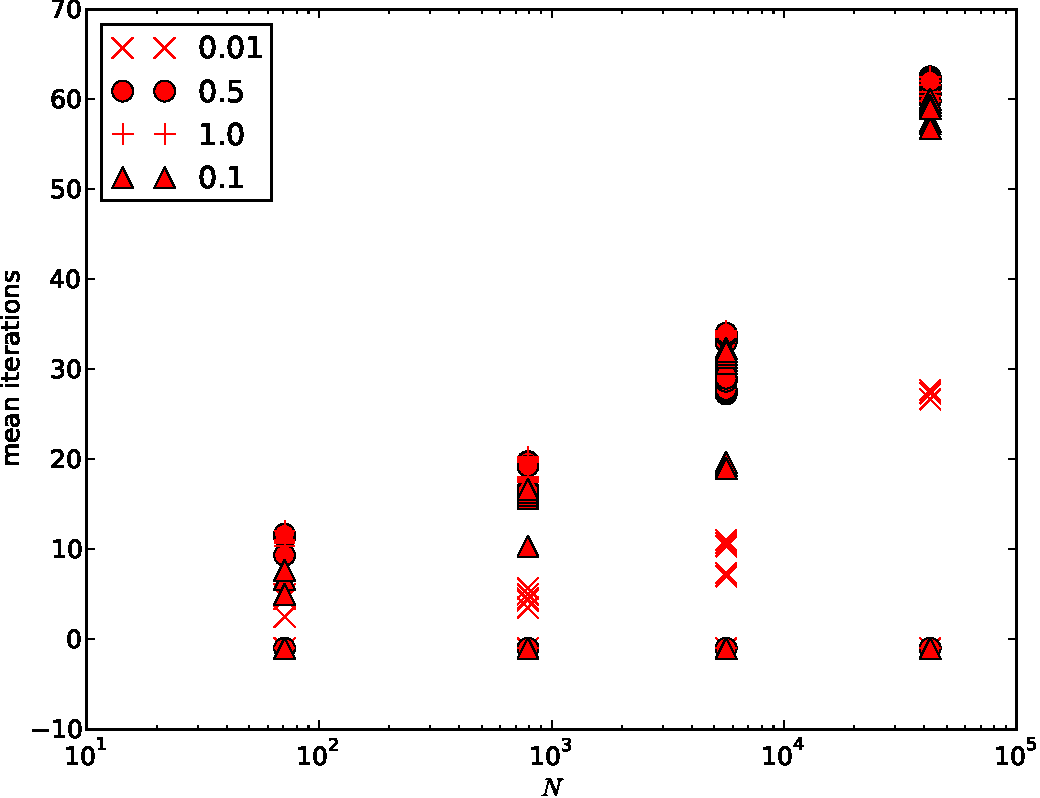
\includegraphics[width=0.8\textwidth]{plots/linear_solvers/ilu-1decoupleddummy-meanofnsolveritersvsinitialnnode.pdf}
  \caption{GMRES iterations to reach relerr $10^{-8}$ for the decoupled LLG preconditioned by ilu-1.}
  \label{fig:its-ilu-decoupled}
\end{figure}

\begin{figure}
  \centering
  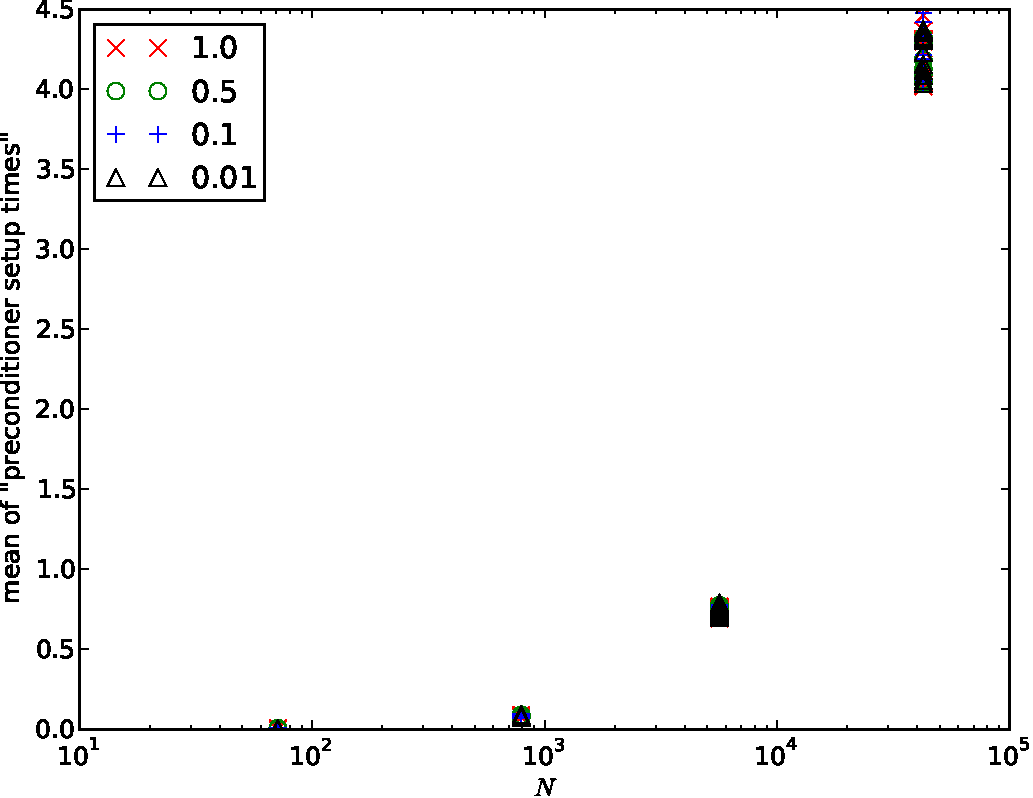
\includegraphics[width=0.8\textwidth]{plots/linear_solvers/ilu-1decoupleddummy-meanofpreconditionersetuptimesvsinitialnnode.pdf}
  \caption{Time to set up an ilu-1 preconditioner for the decoupled LLG block.}
  \label{fig:times-ilu-decoupled}
\end{figure}


Next we consider the preconditioner $\preca$ from \cref{sec:bem-solver-strategies} inverted using a direct solve (LU decomposition).
This is essentially an exact solve without the dense block.
The iteration counts are shown in \cref{fig:its-p1-exact}, they are independent of the number of nodes, time step and all physical parameters.
However the preconditioner setup times, shown in \cref{fig:times-p1-exact} are not so good, as would be expected from a direct solve they grow rapidly for large systems.
Also, due to the direct solve, the memory usage of this preconditioner is large, ran out of space on my machine for largest problem studied.

\begin{figure}
  \centering
  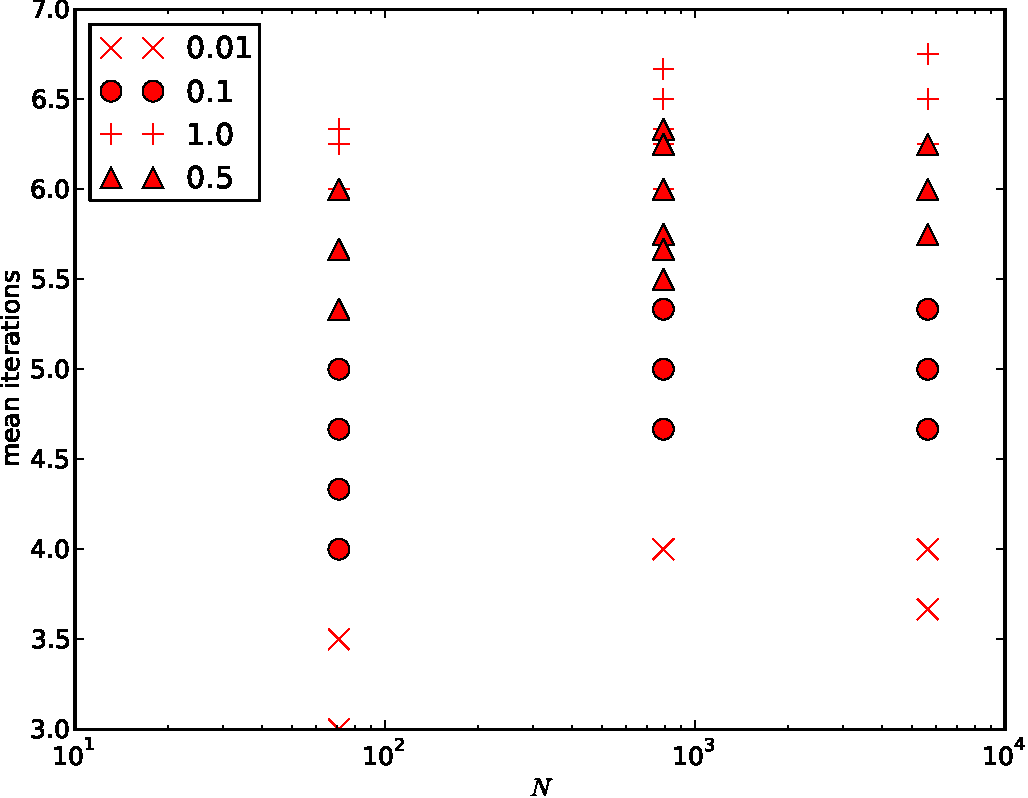
\includegraphics[width=0.8\textwidth]{plots/linear_solvers/som-main-exactimplicitdummy-meanofnsolveritersvsinitialnnode.pdf}
  \caption{Iterations for the monolithic system solved with $\preca$ inverted by LU decomposition.}
  \label{fig:its-p1-exact}
\end{figure}


\begin{figure}
  \centering
  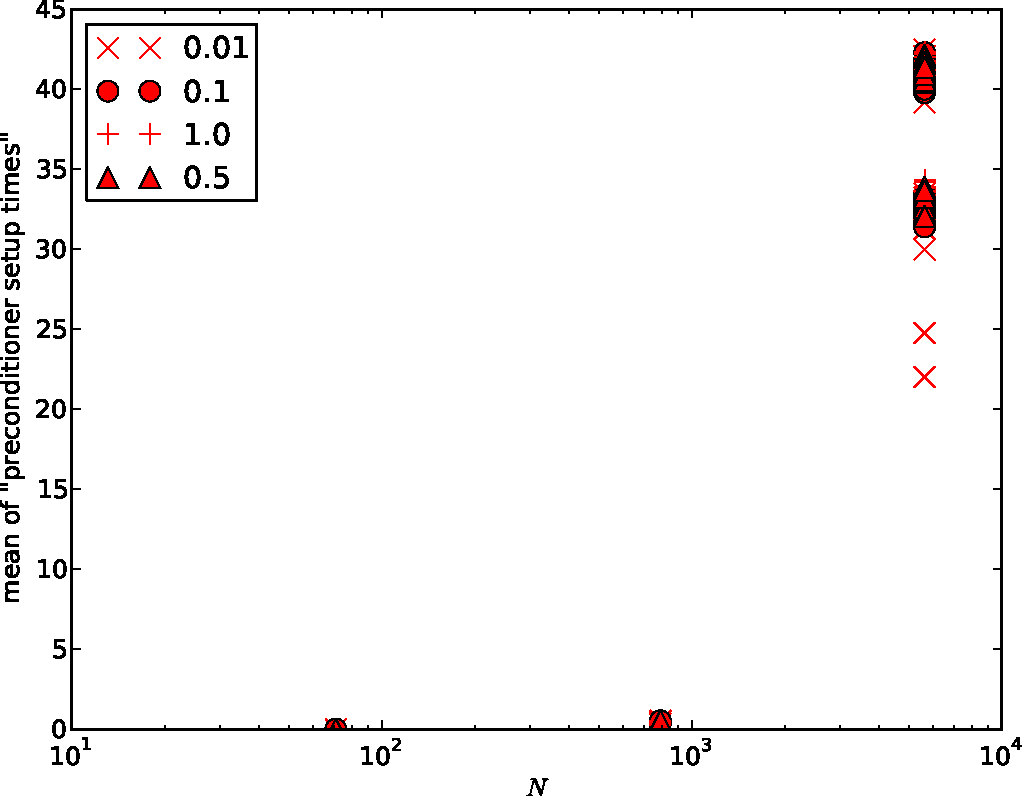
\includegraphics[width=0.8\textwidth]{plots/linear_solvers/som-main-exactimplicitdummy-meanofpreconditionersetuptimesvsinitialnnode.pdf}
  \caption{Preconditioner setup times for $\preca$ inverted by LU decomposition.}
  \label{fig:times-p1-exact}
\end{figure}

The preconditioners $\precb$ and $\precc$ were designed to reduce the setup time.
First we show results for these preconditioners with an exact solve for the $\Fm$ block (and AMG preconditioning, as discussed in \cref{??ds} for the Poisson blocks $\Am$).
The iteration counts are shown in \cref{fig:its-p23-exact}, as with $\preca$ we see that the number of iterations is flat over increasing numbers of nodes, time step size and physical parameters.
The preconditioner setup times are shown in \cref{fig:times-p23-exact}, they are smaller than those in \cref{fig:times-p1-exact} but still grow unacceptably large due to the direct solve of the $\Fm$ block. 

\begin{figure}
  \centering
  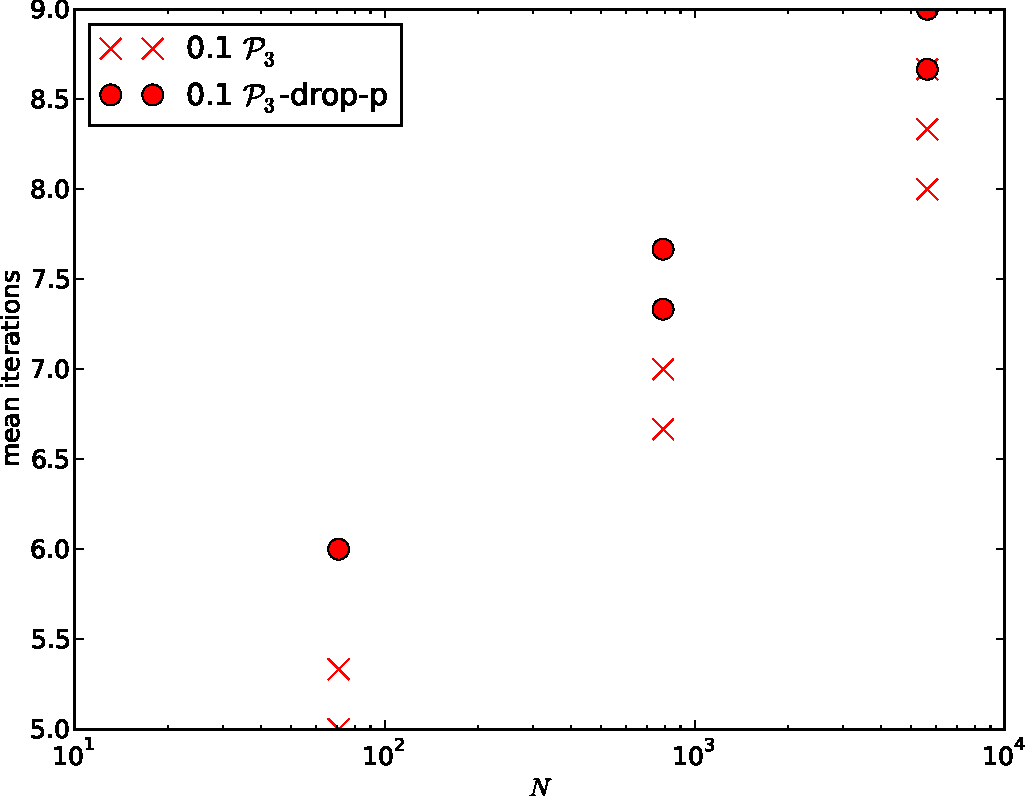
\includegraphics[width=0.8\textwidth]{plots/linear_solvers_p2p3/implicitexact-meanofnsolveritersvsinitialnnode.pdf}
  \caption{Iterations for the monolithic system with $\dtn=0.1$ solved with $\precb$ and $\precc$ with $\Fm$ block inverted by LU decomposition and $\Am$ blocks approximated using AMG.}
  \label{fig:its-p23-exact}
\end{figure}

\begin{figure}
  \centering
  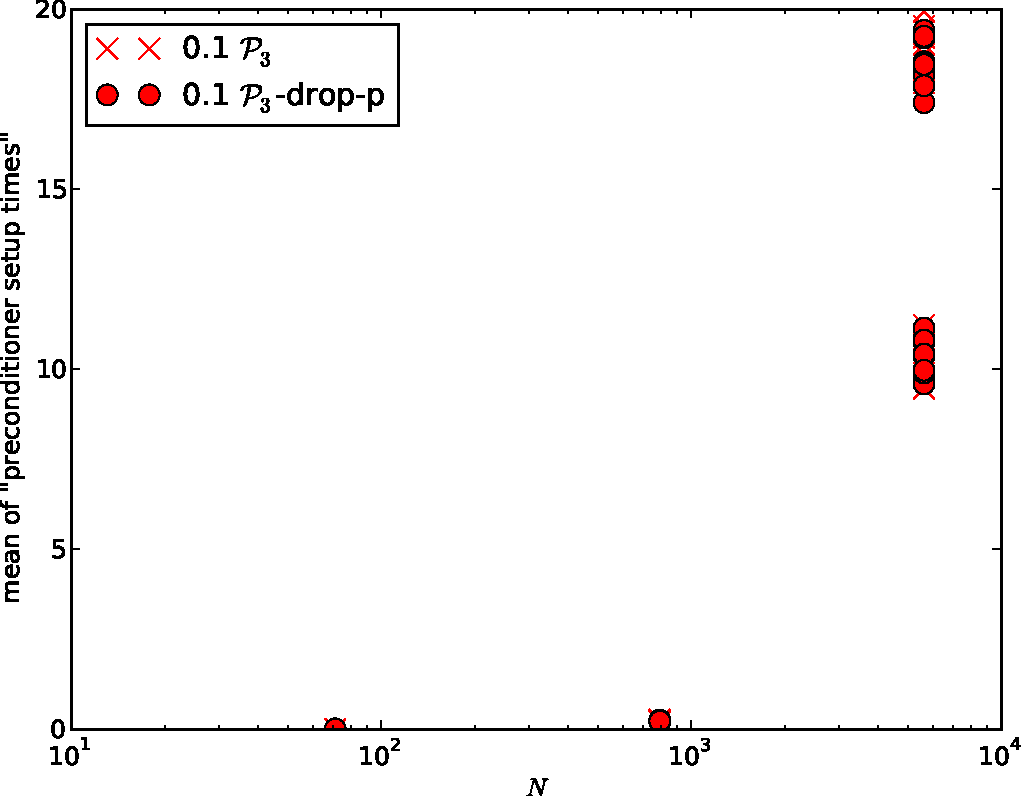
\includegraphics[width=0.8\textwidth]{plots/linear_solvers_p2p3/implicitexact-meanofpreconditionersetuptimesvsinitialnnode.pdf}
  \caption{Preconditioner setup times with $\dtn=0.1$ for $\precb$ and $\precc$ with $\Fm$ block inverted by LU decomposition and $\Am$ blocks approximated using AMG.}
  \label{fig:times-p23-exact}
\end{figure}


Finally we show iteration counts for preconditioners $\precb$ and $\precc$ with the $\Fm$ block solved using the ilu-1 preconditioner.
We cannot expect mesh independent results here, since even the simpler case of the $\Fm$ block alone does not display such behaviour.
The iteration counts shown in \cref{fig:its-p23-ilu1}, are as expected: good at first but ineffective for large meshes.
However the preconditioner set up times, as shown in \cref{fig:times-p23-ilu1} are much better than when using the LU decomposition of the $\Fm$ block. 

\begin{figure}
  \centering
  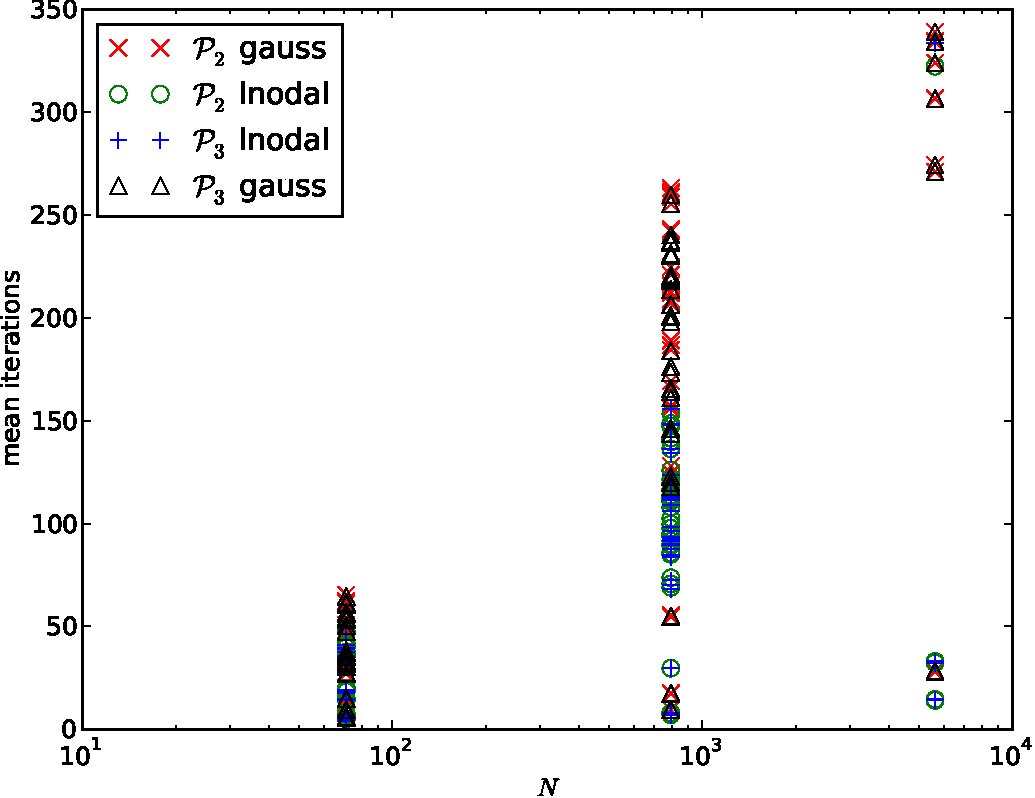
\includegraphics[width=0.8\textwidth]{plots/linear_solvers_p2p3/implicitilu-1-meanofnsolveritersvsinitialnnode.pdf}
  \caption{Iterations for the monolithic system with $\dtn=0.1$ solved with $\precb$ and $\precc$ with $\Fm$ block approximated by ilu-1 and $\Am$ blocks approximated using AMG.}
  \label{fig:its-p23-ilu1}
\end{figure}

\begin{figure}
  \centering
  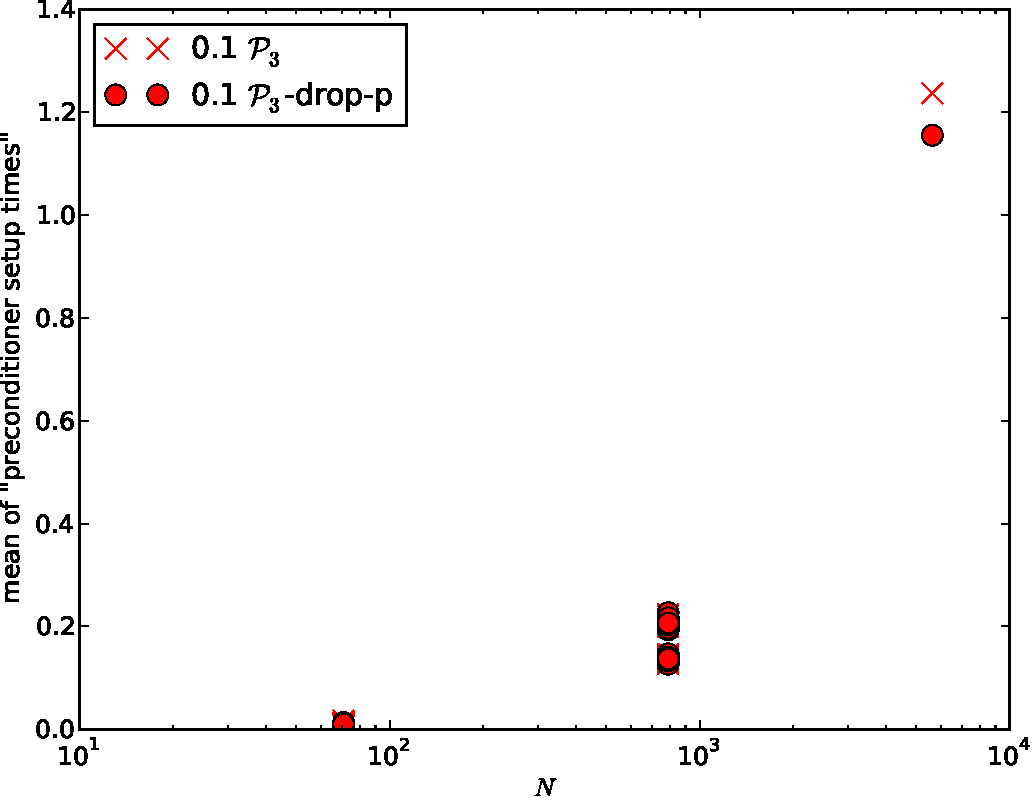
\includegraphics[width=0.8\textwidth]{plots/linear_solvers_p2p3/implicitilu-1-meanofpreconditionersetuptimesvsinitialnnode.pdf}
  \caption{Preconditioner setup times with $\dtn=0.1$ for $\precb$ and $\precc$ with $\Fm$ block approximated by ilu-1 and $\Am$ blocks approximated using AMG.}
  \label{fig:times-p23-ilu1}
\end{figure}

??ds Effect of HLib? If time do this later

Compare the total solve time for the semi-implicit method (with GMRES and ilu-1 preconditioning) and fully implicit method (with $\precb$, ilu-1 for the $\Fm$ block), both using HLib.
Results are shown in \cref{fig:times-semi-vs-fully-implicit}.
??ds fully implicit a bit slower but not horrible..
Note that in our current implementation the Jacobian assembly time for the fully implicit method is longer than that of the semi-implicit one, however this does not need to be the case with some simple optimisations discussed in \cref{sec:furth-optim-opport}.

\begin{figure}
  \centering
  
\includegraphics[width=0.8\textwidth]{images/placeholder}
  \caption{}
  \label{fig:times-semi-vs-fully-implicit}
\end{figure}


Jacobian assembly times? -- probably not, since not representative of ``real'' situation



\section{Outlook}
\label{sec:furth-optim-opport}

In this \thisref{sec:furth-optim-opport} we compare the expected performance of the fully implicit and decoupled approaches with the assumption that a ``sufficiently good'' preconditioner for the $\Fm$ block can be found and discuss further improvements that could be made.

In the fully implicit method timing results presented here the entire FEM Jacobian was recalculated at each Newton step.
This is not actually necessary: the Poisson blocks, $\Am$, and LLG-Poisson coupling blocks, $\Qm$ and $\Pm$, (of \cref{eq:16}) are only dependent on the geometry (\ie the corresponding equations are linear).
Hence these blocks could be precomputed and stored.
This reduces the Jacobian assembly process for the fully implicit method to exactly as the decoupled method.

Similarly the mass matrix sub-blocks on the diagonal of the LLG-block ($\Mm$ of \cref{eq:llg-jacobian}) are only dependent on the geometry.
As an additional optimisation the skew symmetric structure of \cref{eq:llg-jacobian} could be exploited so that the calculation of $\Km_x$ is reused for $-\Km_x$, and similarly for $\Km_y$ and $\Km_z$.
Applying these additional optimisations will reduce the Jacobian calculations to the assembly of three $N \times N$ Jacobian blocks and the magnetocrystalline anisotropy block (which will typically be either $N \times N$ or empty).


Newton residual assembly time is extremely small compared to solve + Jacobian assembly times, so it will be ignored.

So the solve time difference is all that is left: both using Krylov solvers, but fully coupled has extra non-zeros (P, Q, G blocks), approx $4N$ extra elements (base is $11N$), hence approximately half as much time again needed for each Krylov step.
Also fully coupled must use GMRES for all blocks, rather than only for $\Fm$: potentially more expensive orthogonalisation process, could possibly be removed by switching to BiCGStab.
Finally: possible additional iterations, depends on preconditioner used.




More effective mesh preconditioners for the $\Fm$ block are badly needed.
For granular or bit patterned media a domain-decomposition preconditioner exploiting the low/zero exchange coupling between grains/islands could be extremely effective.
Such a preconditioner could be implemented by using a direct solve on each grain/island and using this diagonal block solution as the preconditioner.

Reordering of the degrees of freedom, scaling, drop tolerance, fill-in level... of the ILU preconditioner could be experimented with to allow somewhat larger systems \cite[287]{Saad2000}.
But ILU is very unlikely to ever give mesh independent iteration counts 


\section{Conclusions}

We have demonstrated a fully implicit solver using preconditioned GMRES which is close in terms of cost per linear solve.

For small meshes and/or time steps ILU-1 is a good preconditioner for the LLG block.

Effective mesh independent preconditioners for the $\Fm$ block are badly needed.

AMG and dropping either P or Q is an excellent preconditioner for the Poisson blocks: almost no increase in number of iterations compared to exact!



%%% Local Variables:
%%% mode: latex
%%% TeX-master: "main"
%%% End:
